\section{Experiments  }

\subsection{Setup}

For the experiments, we evaluated our implementation using different temporal constraints and initial states on the the simplified $\asprilo$ domain. The presented results ran using $\clingo$ 5.4.0 on an Intel Xeon E5-2650v4 under Debian GNU/Linux 9, with a memory of 20 GB and a timeout of 20 min per instance.

Throughout the experiments, we use three temporal constraints to limit the movements of robots. These constraints make use of additional predicates, which are included as part of the planning encoding. The first constraint is shown in Listing 19 and it restricts robots to move vertically before horizontally (allowing pauses between movements). Such constraint corresponds to the temporal formula $\neg\; \mathit{move\_horizontally(robot(R))} \until (\alwaysF \;\neg \;\mathit{move\_vertically(robot(R)))}$.

\begin{center}
    \begin{lstlisting}[] 
:- not &tel{(~ move_horizontally(robot(R)) ) >? 
                (>* ~ move_vertically(robot(R))) },
    robot(R).
    \end{lstlisting}
\captionof{lstlisting}{Move vertically before horizontally in $\LTLf$ .}
\end{center}

We can also express this constraint in $\LDLf$ using the equivalent formula \\ $\deventually{ (\mathit{no\_move\_horizontally(robot(R))} ; \top)^\ast} \dalways{\top^\ast} \mathit{no\_move\_vertically(robot(R))}$. \\The integration of predicates \texttt{no\_move\_horizontally/1} and \texttt{no\_move\_vertically/1} into the encoding is necessary to account for the aforementioned restrictions on this logic.

\begin{center}
    \begin{lstlisting}[] 
:- not &del{ *( ? no_move_horizontally(robot(R)) ;; &true ) .>? 
             ( (* &true ) .>* no_move_vertically(robot(R)) )}, 
    robot(R).
    \end{lstlisting}
\captionof{lstlisting}{Move vertically before horizontally in $\LDLf$ .}
\end{center}

The constraint to enforce horizontal movements before vertical ones is defined analogously to Listing 19 and Listing 20. For the last constraint, we ensure that robots move only in one direction in the x axis (right or left) and in one direction in the y axis (up or down). 

\begin{center}
    \begin{lstlisting}[] 
:- not &tel{ (>* (~ move_right(robot(R)))) |  
             (>* (~ move_left(robot(R)))) }, 
    robot(R).

:- not &tel{ (>* (~ move_up(robot(R)))) |  
             (>* (~ move_down(robot(R)))) }, 
    robot(R).
    \end{lstlisting}
\captionof{lstlisting}{Never both directions in $\LTLf$.}
\end{center}

By applying the equivalences for each operator we can translate the first formula in Listing 20 to one on $\LDLf$, namely $\deventually{(\dalways{\top^\ast}~move\_right(robot(R)))? + (\dalways{\top^\ast}~move\_left(robot(R)))?}\top$. This formula, however, does not follow our restrictions given that the test construct is applied to a formula with the box operator. Therefore, this constraint required some adjustments to be written under our specification, yielding the encoding in Listing 22.


\begin{center}
    \begin{lstlisting}[] 
:- not &del{ *(&true ;; ? no_move_right(robot(R))) +
             *(&true ;; ? no_move_left(robot(R))) .>?
             (&true.>* &false) }, 
    robot(R).

:- not &del{ *(&true ;; ? no_move_up(robot(R))) +
            *(&true ;; ? no_move_down(robot(R))) .>?
            (&true.>* &false) }, 
robot(R).
    \end{lstlisting}
\captionof{lstlisting}{Never both directions in $\LDLf$.}
\end{center}

Regarding the planning instances, we consider warehouses defined by configurations varying in size and number of robots. In the presented results, we follow the naming format for $\asprilo$ instances, where name \textit{xN\_yM\_rO} refers to instances of grid size $N\times M$ with $O$ robots.  
We also explored two different types of arrangements of the warehouse. A \emph{structured} one, where the robots are always in the lower left corner (Figure 4), as well as a second one, called \emph{grid} where robots are scattered in the space and obstacles can be present (Figure 5). 
For each configuration, we contemplate five initial states differing on the position of the destinations, represented by the last two numbers of the instance name.


\begin{figure}
    \centering
\begin{subfigure}{.45\textwidth}
    \centering
    \includegraphics[scale=0.18]{img/g-asprilo-nc.png}
    \caption{Movement of robots without constraint.}
\end{subfigure}%
\hspace{10px}
\begin{subfigure}{.45\textwidth}
    \centering
    \includegraphics[scale=0.18]{img/g-asprilo.png}
    \caption{Applying constraint of never both directions.}
\end{subfigure}
\caption{Asprilo visualization for grid instance g-x5\_y5\_n20\_r5-05 with horizon 5, where cells in black represent obstacles.}
\end{figure}

\subsection{Results}


In the following results, we compare our implementation using automata from temporal and dynamic formulas against the encoding without these additional constraints, refereed to as `nc'. As baseline, we use a translation of the integrity constraints in $\LTLf$ to plain ASP trough $\TELf$, in the same way as in $\telingo$ \cite{cakamosc19a}. We use the name `asp' to refer to this last approach.

First, we present the most significant results encountered regarding the solving times of each method when searching for all the stable models of the program. In Figure 6, we can notice that, as expected, solving times are reduced drastically when applying a new integrity constraint to the program. In the case of no constraint, the solver reaches a timeout for all instances and constraints. Furthermore, the performance of the approach using $\LTLf$ is overall better than that for $\LDLf$. This behavior can be due to the different representation of states, either by numbers or predicates, between both methods. Moreover, it can be related to the differences of the translation of formulas. Overall, our baseline persist being considerably faster.



\begin{figure}[]
    \centering
    
    % This file was created by tikzplotlib v0.9.3.
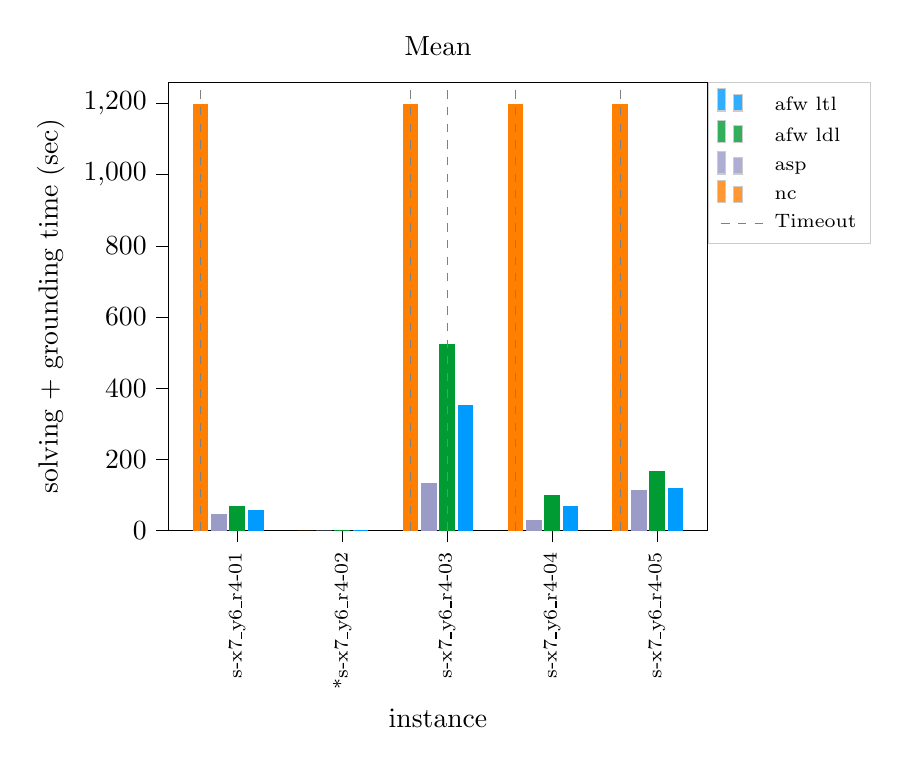
\begin{tikzpicture}

    \definecolor{color0}{rgb}{0,0.607843137254902,1}
    \definecolor{color1}{rgb}{0,0.607843137254902,0.2}
    \definecolor{color2}{rgb}{0.607843137254902,0.607843137254902,0.784313725490196}
    \definecolor{color3}{rgb}{1,0.498039215686275,0}
    
    \begin{axis}[
    legend cell align={left},
    legend style={font=\scriptsize,fill opacity=0.8, draw opacity=1, text opacity=1, at={(1,1)}, anchor=north west, draw=white!80!black},
    tick align=outside,
    tick pos=left,
    title={Mean},
    x grid style={white!69.0196078431373!black},
    xlabel={instance},
    xmin=-0.65875, xmax=4.48375,
    xtick style={color=black},
    xtick={0,1,2,3,4},
    xticklabel style = {font=\scriptsize,rotate=90.0},
    xticklabels={s-x7\_y6\_r4-01,*s-x7\_y6\_r4-02,s-x7\_y6\_r4-03,s-x7\_y6\_r4-04,s-x7\_y6\_r4-05},
    y grid style={white!69.0196078431373!black},
    ylabel={solving + grounding time (sec)},
    ymin=0, ymax=1260.01051025391,
    ytick style={color=black}
    ]
    \draw[draw=none,fill=color0] (axis cs:0.25,0) rectangle (axis cs:0.1,57.9530029296875);
    \addlegendimage{ybar,ybar legend,draw=none,fill=color0};
    \addlegendentry{afw ltl}
    
    \draw[draw=none,fill=color0] (axis cs:1.25,0) rectangle (axis cs:1.1,0.0643333345651627);
    \draw[draw=none,fill=color0] (axis cs:2.25,0) rectangle (axis cs:2.1,353.798980712891);
    \draw[draw=none,fill=color0] (axis cs:3.25,0) rectangle (axis cs:3.1,67.5556640625);
    \draw[draw=none,fill=color0] (axis cs:4.25,0) rectangle (axis cs:4.1,120.026000976562);
    \draw[draw=none,fill=color1] (axis cs:0.075,0) rectangle (axis cs:-0.075,68.9150009155273);
    \addlegendimage{ybar,ybar legend,draw=none,fill=color1};
    \addlegendentry{afw ldl}
    
    \draw[draw=none,fill=color1] (axis cs:1.075,0) rectangle (axis cs:0.925,0.0816666707396507);
    \draw[draw=none,fill=color1] (axis cs:2.075,0) rectangle (axis cs:1.925,524.588317871094);
    \draw[draw=none,fill=color1] (axis cs:3.075,0) rectangle (axis cs:2.925,98.8453369140625);
    \draw[draw=none,fill=color1] (axis cs:4.075,0) rectangle (axis cs:3.925,166.195343017578);
    \draw[draw=none,fill=color2] (axis cs:-0.1,0) rectangle (axis cs:-0.25,47.4580039978027);
    \addlegendimage{ybar,ybar legend,draw=none,fill=color2};
    \addlegendentry{asp}
    
    \draw[draw=none,fill=color2] (axis cs:0.9,0) rectangle (axis cs:0.75,0.0489999987185001);
    \draw[draw=none,fill=color2] (axis cs:1.9,0) rectangle (axis cs:1.75,132.566665649414);
    \draw[draw=none,fill=color2] (axis cs:2.9,0) rectangle (axis cs:2.75,30.5513324737549);
    \draw[draw=none,fill=color2] (axis cs:3.9,0) rectangle (axis cs:3.75,114.831665039062);
    \draw[draw=none,fill=color3] (axis cs:-0.275,0) rectangle (axis cs:-0.425,1199.98498535156);
    \addlegendimage{ybar,ybar legend,draw=none,fill=color3};
    \addlegendentry{nc}
    
    \draw[draw=none,fill=color3] (axis cs:0.725,0) rectangle (axis cs:0.575,0.0260000005364418);
    \draw[draw=none,fill=color3] (axis cs:1.725,0) rectangle (axis cs:1.575,1200.01000976562);
    \draw[draw=none,fill=color3] (axis cs:2.725,0) rectangle (axis cs:2.575,1200.0009765625);
    \draw[draw=none,fill=color3] (axis cs:3.725,0) rectangle (axis cs:3.575,1199.98596191406);
    \addplot [line width=0.28pt, white!50.1960784313725!black, dashed]
    table {%
    2 2.8421709430404e-14
    2 1260.01051025391
    };
    \addlegendentry{Timeout}
    \addplot [line width=0.28pt, white!50.1960784313725!black, dashed]
    table {%
    -0.35 2.8421709430404e-14
    -0.35 1260.01051025391
    };
    \addplot [line width=0.28pt, white!50.1960784313725!black, dashed]
    table {%
    1.65 2.8421709430404e-14
    1.65 1260.01051025391
    };
    \addplot [line width=0.28pt, white!50.1960784313725!black, dashed]
    table {%
    2.65 2.8421709430404e-14
    2.65 1260.01051025391
    };
    \addplot [line width=0.28pt, white!50.1960784313725!black, dashed]
    table {%
    3.65 2.8421709430404e-14
    3.65 1260.01051025391
    };
    \end{axis}
    
    \end{tikzpicture}
    
    \caption{Average of solving and grounding times for all three constraint with horizon 7 when obtaining all models in $\clingo$. Unsatisfiable instances are marked with *.}
\end{figure}

A higher horizon was required for bigger instances to become satisfiable, however, increasing the horizon led mostly to timeouts. Thus, we used clingo to compute only one model in order to examine more details about the programs for such larger instances. In Figure 7, we show the size of the program w.r.t. the number of rules and bodies with horizon 20. This figure presents instances grouping all initial states of each configuration. The proportion of rules and bodies remains proportional throughout the experiment, indicating that while programs increased in size of the new encoding, this was done by the same amount of rules as bodies. 
% Therefore, there was no special increase in facts.
We can also notice a minimal increase in size of the program when using the translation to ASP, whereas the introduction of the automata encoding almost doubles the original size.

\begin{figure}[]
    \centering
    
    % This file was created by tikzplotlib v0.9.3.
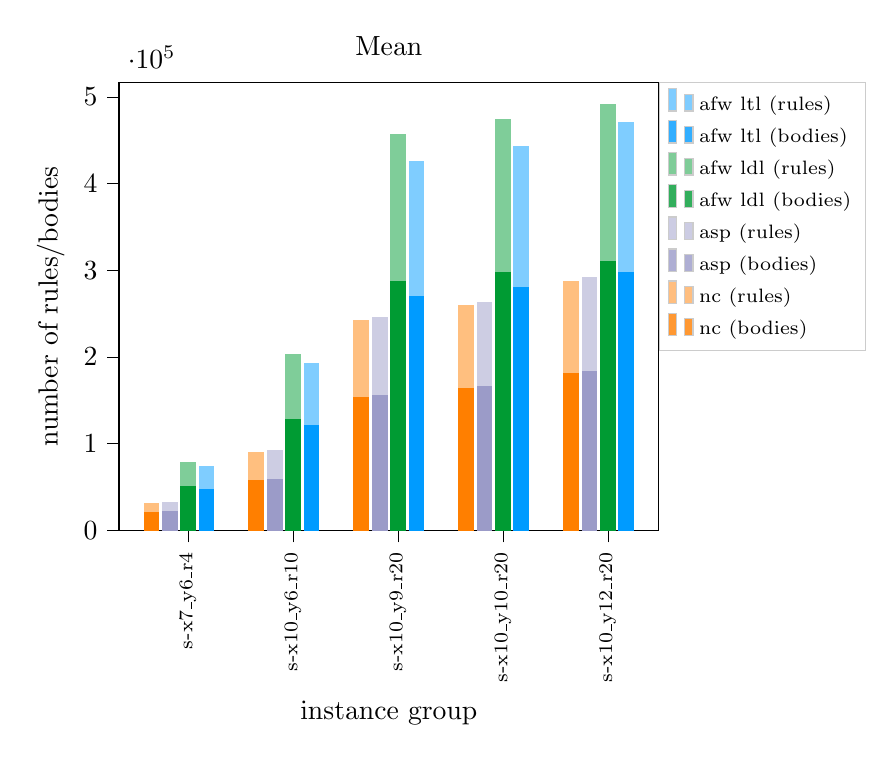
\begin{tikzpicture}

    \definecolor{color0}{rgb}{0,0.607843137254902,1}
    \definecolor{color1}{rgb}{0,0.607843137254902,0.2}
    \definecolor{color2}{rgb}{0.607843137254902,0.607843137254902,0.784313725490196}
    \definecolor{color3}{rgb}{1,0.498039215686275,0}
    
    \begin{axis}[
    legend cell align={left},
    legend style={font=\scriptsize,fill opacity=0.8, draw opacity=1, text opacity=1, at={(1,1)}, anchor=north west, draw=white!80!black},
    tick align=outside,
    tick pos=left,
    title={Mean},
    x grid style={white!69.0196078431373!black},
    xlabel={instance group},
    xmin=-0.65875, xmax=4.48375,
    xtick style={color=black},
    xtick={0,1,2,3,4},
    xticklabel style = {font=\scriptsize,rotate=90.0},
    xticklabels={s-x7\_y6\_r4,s-x10\_y6\_r10,s-x10\_y9\_r20,s-x10\_y10\_r20,s-x10\_y12\_r20},
    y grid style={white!69.0196078431373!black},
    ylabel={number of rules/bodies},
    ymin=0, ymax=516864.6,
    ytick style={color=black}
    ]
    \draw[draw=none,fill=color0,fill opacity=0.5] (axis cs:0.25,0) rectangle (axis cs:0.1,74920.3359375);
    \addlegendimage{ybar,ybar legend,draw=none,fill=color0,fill opacity=0.5};
    \addlegendentry{afw ltl (rules)}
    
    \draw[draw=none,fill=color0,fill opacity=0.5] (axis cs:1.25,0) rectangle (axis cs:1.1,192576);
    \draw[draw=none,fill=color0,fill opacity=0.5] (axis cs:2.25,0) rectangle (axis cs:2.1,426149.65625);
    \draw[draw=none,fill=color0,fill opacity=0.5] (axis cs:3.25,0) rectangle (axis cs:3.1,443255.65625);
    \draw[draw=none,fill=color0,fill opacity=0.5] (axis cs:4.25,0) rectangle (axis cs:4.1,471535.34375);
    \draw[draw=none,fill=color0] (axis cs:0.25,0) rectangle (axis cs:0.1,48106);
    \addlegendimage{ybar,ybar legend,draw=none,fill=color0};
    \addlegendentry{afw ltl (bodies)}
    
    \draw[draw=none,fill=color0] (axis cs:1.25,0) rectangle (axis cs:1.1,121728);
    \draw[draw=none,fill=color0] (axis cs:2.25,0) rectangle (axis cs:2.1,269848.34375);
    \draw[draw=none,fill=color0] (axis cs:3.25,0) rectangle (axis cs:3.1,280269);
    \draw[draw=none,fill=color0] (axis cs:4.25,0) rectangle (axis cs:4.1,297466.65625);
    \draw[draw=none,fill=color1,fill opacity=0.5] (axis cs:0.075,0) rectangle (axis cs:-0.075,79077);
    \addlegendimage{ybar,ybar legend,draw=none,fill=color1,fill opacity=0.5};
    \addlegendentry{afw ldl (rules)}
    
    \draw[draw=none,fill=color1,fill opacity=0.5] (axis cs:1.075,0) rectangle (axis cs:0.925,202942.671875);
    \draw[draw=none,fill=color1,fill opacity=0.5] (axis cs:2.075,0) rectangle (axis cs:1.925,456794);
    \draw[draw=none,fill=color1,fill opacity=0.5] (axis cs:3.075,0) rectangle (axis cs:2.925,473870);
    \draw[draw=none,fill=color1,fill opacity=0.5] (axis cs:4.075,0) rectangle (axis cs:3.925,492252);
    \draw[draw=none,fill=color1] (axis cs:0.075,0) rectangle (axis cs:-0.075,50756.66796875);
    \addlegendimage{ybar,ybar legend,draw=none,fill=color1};
    \addlegendentry{afw ldl (bodies)}
    
    \draw[draw=none,fill=color1] (axis cs:1.075,0) rectangle (axis cs:0.925,128354.6640625);
    \draw[draw=none,fill=color1] (axis cs:2.075,0) rectangle (axis cs:1.925,288035.34375);
    \draw[draw=none,fill=color1] (axis cs:3.075,0) rectangle (axis cs:2.925,298441.34375);
    \draw[draw=none,fill=color1] (axis cs:4.075,0) rectangle (axis cs:3.925,310720);
    \draw[draw=none,fill=color2,fill opacity=0.5] (axis cs:-0.1,0) rectangle (axis cs:-0.25,32725);
    \addlegendimage{ybar,ybar legend,draw=none,fill=color2,fill opacity=0.5};
    \addlegendentry{asp (rules)}
    
    \draw[draw=none,fill=color2,fill opacity=0.5] (axis cs:0.9,0) rectangle (axis cs:0.75,92716.3359375);
    \draw[draw=none,fill=color2,fill opacity=0.5] (axis cs:1.9,0) rectangle (axis cs:1.75,246315.328125);
    \draw[draw=none,fill=color2,fill opacity=0.5] (axis cs:2.9,0) rectangle (axis cs:2.75,263481.34375);
    \draw[draw=none,fill=color2,fill opacity=0.5] (axis cs:3.9,0) rectangle (axis cs:3.75,291792.34375);
    \draw[draw=none,fill=color2] (axis cs:-0.1,0) rectangle (axis cs:-0.25,22262.666015625);
    \addlegendimage{ybar,ybar legend,draw=none,fill=color2};
    \addlegendentry{asp (bodies)}
    
    \draw[draw=none,fill=color2] (axis cs:0.9,0) rectangle (axis cs:0.75,59867.33203125);
    \draw[draw=none,fill=color2] (axis cs:1.9,0) rectangle (axis cs:1.75,156003);
    \draw[draw=none,fill=color2] (axis cs:2.9,0) rectangle (axis cs:2.75,166453);
    \draw[draw=none,fill=color2] (axis cs:3.9,0) rectangle (axis cs:3.75,183666);
    \draw[draw=none,fill=color3,fill opacity=0.5] (axis cs:-0.275,0) rectangle (axis cs:-0.425,32003);
    \addlegendimage{ybar,ybar legend,draw=none,fill=color3,fill opacity=0.5};
    \addlegendentry{nc (rules)}
    
    \draw[draw=none,fill=color3,fill opacity=0.5] (axis cs:0.725,0) rectangle (axis cs:0.575,90911);
    \draw[draw=none,fill=color3,fill opacity=0.5] (axis cs:1.725,0) rectangle (axis cs:1.575,242698);
    \draw[draw=none,fill=color3,fill opacity=0.5] (axis cs:2.725,0) rectangle (axis cs:2.575,259864);
    \draw[draw=none,fill=color3,fill opacity=0.5] (axis cs:3.725,0) rectangle (axis cs:3.575,288175);
    \draw[draw=none,fill=color3] (axis cs:-0.275,0) rectangle (axis cs:-0.425,21771);
    \addlegendimage{ybar,ybar legend,draw=none,fill=color3};
    \addlegendentry{nc (bodies)}
    
    \draw[draw=none,fill=color3] (axis cs:0.725,0) rectangle (axis cs:0.575,58638);
    \draw[draw=none,fill=color3] (axis cs:1.725,0) rectangle (axis cs:1.575,153541);
    \draw[draw=none,fill=color3] (axis cs:2.725,0) rectangle (axis cs:2.575,163991);
    \draw[draw=none,fill=color3] (axis cs:3.725,0) rectangle (axis cs:3.575,181204);
    \end{axis}
    
    \end{tikzpicture}
    
    \caption{Average number of rules and bodies for all three constraint with horizon 20 when obtaining one model. Instances are grouped by configuration. }
\end{figure}


Next, we decided to inspect the scalability of the implementation for both temporal and dynamic logic. This was done by increasing the horizon and asking only for the first model. The results are shown in Figure 8 and show a similar behavior between both models. Interestingly, the solving time for the dynamic formulas is only better on the instances with the configuration of $10\times 10$ and 20 robots.


\begin{figure}[]
    \centering
    
    % This file was created by tikzplotlib v0.9.3.
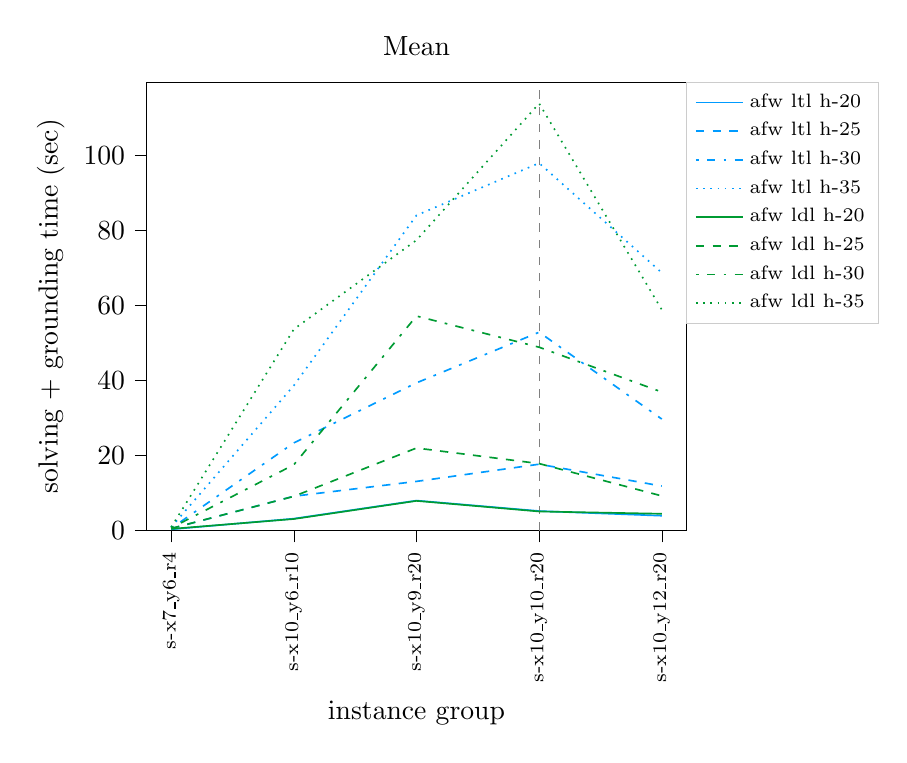
\begin{tikzpicture}

    \definecolor{color0}{rgb}{0,0.607843137254902,1}
    \definecolor{color1}{rgb}{0,0.607843137254902,0.2}
    
    \begin{axis}[
    legend cell align={left},
    legend style={font=\scriptsize,fill opacity=0.8, draw opacity=1, text opacity=1, at={(1,1)}, anchor=north west, draw=white!80!black},
    tick align=outside,
    tick pos=left,
    title={Mean},
    x grid style={white!69.0196078431373!black},
    xlabel={instance group},
    xmin=-0.2, xmax=4.2,
    xtick style={color=black},
    xtick={0,1,2,3,4},
    xticklabel style = {font=\scriptsize,rotate=90.0},
    xticklabels={s-x7\_y6\_r4,s-x10\_y6\_r10,s-x10\_y9\_r20,s-x10\_y10\_r20,s-x10\_y12\_r20},
    y grid style={white!69.0196078431373!black},
    ylabel={solving + grounding time (sec)},
    ymin=0, ymax=119.437843351066,
    ytick style={color=black}
    ]
    \addplot [semithick, color0, opacity=1]
    table {%
    0 0.327666670084
    1 3.15793347358704
    2 7.97200012207031
    3 5.18893337249756
    4 3.93733334541321
    };
    \addlegendentry{afw ltl h-20}
    \addplot [line width=0.28pt, white!50.1960784313725!black, dashed, forget plot]
    table {%
    3 3.5527136788005e-15
    3 119.437843351066
    };
    \addplot [semithick, color0, opacity=1, dashed]
    table {%
    0 0.508133351802826
    1 9.13133335113525
    2 13.082667350769
    3 17.6627330780029
    4 11.8399991989136
    };
    \addlegendentry{afw ltl h-25}
    \addplot [semithick, color0, opacity=1, dash pattern=on 1pt off 3pt on 3pt off 3pt]
    table {%
    0 0.570133328437805
    1 23.3456649780273
    2 39.3339996337891
    3 52.8310050964355
    4 29.6908664703369
    };
    \addlegendentry{afw ltl h-30}
    \addplot [semithick, color0, opacity=1, dotted]
    table {%
    0 0.892533302307129
    1 38.6154670715332
    2 83.9641952514648
    3 97.8827285766602
    4 68.6672668457031
    };
    \addlegendentry{afw ltl h-35}
    \addplot [semithick, color1, opacity=1]
    table {%
    0 0.427333325147629
    1 3.07173347473145
    2 7.8985333442688
    3 5.07393312454224
    4 4.45966672897339
    };
    \addlegendentry{afw ldl h-20}
    \addplot [semithick, color1, opacity=1, dashed]
    table {%
    0 0.549266636371613
    1 9.10186672210693
    2 21.9740009307861
    3 17.8249340057373
    4 9.21719932556152
    };
    \addlegendentry{afw ldl h-25}
    \addplot [semithick, color1, opacity=1, dash pattern=on 1pt off 3pt on 3pt off 3pt]
    table {%
    0 0.688400030136108
    1 17.520601272583
    2 57.1371955871582
    3 48.8288612365723
    4 36.8923301696777
    };
    \addlegendentry{afw ldl h-30}
    \addplot [semithick, color1, opacity=1, dotted]
    table {%
    0 0.884466648101807
    1 53.6264686584473
    2 77.3668670654297
    3 113.765930175781
    4 58.8269348144531
    };
    \addlegendentry{afw ldl h-35}
    \end{axis}
    
    \end{tikzpicture}
    
    \caption{Average solving times for all three constraint with horizons 20 to 35, when obtaining one model. Instances are grouped by configuration. }
\end{figure}


For our last analysis, we examined the number of choices and conflicts found by the solver for each approach. This was done for instances using the grid configuration. Results on Table 3 correspond to the number of conflicts when computing all models with a horizon of 5. 
Unlike the rest of the analysis, we here show the results only for the constraint ensuring robots do not move in both directions (listings 21 and 22). 
As we can observe in Table 3, the numbers decreased in over one order of magnitude for all satisfiable instances. 
Particularly, in the case of instance $g-x5\_y5\_n20\_r5-05$ (Figure 5), where 5 obstacles are presented\footnote{The number of obstacles is calculated based on the name as follows: $O=X\times Y-N$}, we can see a drastical improvement. Some of the presented instances become unsatisfied when including the constraints, due to the presence of obstacles which can only be avoided by moving in both directions. Furthermore, the number of conflicts is reduced in half when using temporal instead of dynamic logic.
A similar evaluation was performed for the number of choices in the program (Table 4). Here we recognize the same type of reduction. Although, in this case, the difference of choices between both logics is not as evident. As final remarks on these results, we notice an improvement on the use of the automata approach against our baseline for the first two instances. However, this gain is not encountered in the rest of the experiments.






\begin{table}
\centering
\begin{tabular}{|l|r|r|r|r|r|r|r|r|}
    \hline
    {} &  \textbf{afw ltl}&    \textbf{afw ldl} &    \textbf{asp} &    \textbf{nc}  \\
    \hline
    g-x5\_y5\_n20\_r5-01 &                        162 &                            340 &                        366 &                      7713 \\
    g-x5\_y5\_n20\_r5-02 &                         87 &                             64 &                        102 &                       218 \\
    g-x5\_y5\_n20\_r5-03 &                          1* &                              1* &                          1* &                         1* \\
    g-x5\_y5\_n20\_r5-04 &                       6511 &                          13428 &                       1348 &                    153447 \\
    g-x5\_y5\_n20\_r5-05 &                      13972 &                          62683 &                       5967 &                   6871918 \\
    \hline
    \hline
    g-x5\_y5\_n25\_r5-01 &                     115477 &                         242147 &                      62126 &                  11891485 \\
    g-x5\_y5\_n25\_r5-02 &                          1* &                              1* &                          1* &                         1* \\
    g-x5\_y5\_n25\_r5-03 &                     287504 &                         716067 &                     166992 &                  23184916 \\
    g-x5\_y5\_n25\_r5-04 &                         22* &                             25* &                         29* &                   3490969 \\
    g-x5\_y5\_n25\_r5-05 &                          1* &                              1* &                          1* &                         1* \\
    \bottomrule
    \end{tabular}
    
\caption{Number of conflicts with horizon 5 obtaining all models of instances in the grid configuration for constraint "never both directions". Results marked with * refer to unsatisfiable status. Instances in the first half of the table have 5 obstacle, whereas the ones in the bottom half have none.}
\end{table}


\begin{table}
\centering

    \begin{tabular}{|l|r|r|r|r|r|r|r|r|}
% \toprule
\hline
{} &  \textbf{afw ltl}&    \textbf{afw ldl} &    \textbf{asp} &    \textbf{nc}  \\
% \midrule
\hline

g-x5\_y5\_n20\_r5-01 &                     1367 &                         1548 &                      976 &                   17884 \\
g-x5\_y5\_n20\_r5-02 &                      292 &                          273 &                      212 &                    1240 \\
g-x5\_y5\_n20\_r5-03 &                        0* &                            0* &                        0* &                       0* \\
g-x5\_y5\_n20\_r5-04 &                    51338 &                        58250 &                     4189 &                 1065833 \\
g-x5\_y5\_n20\_r5-05 &                   109212 &                       157972 &                    17941 &                26319932 \\ 
\hline
\hline
g-x5\_y5\_n25\_r5-01 &                  1027511 &                      1154285 &                   290203 &                35869208 \\
g-x5\_y5\_n25\_r5-02 &                        0* &                            0* &                        0* &                       0* \\
g-x5\_y5\_n25\_r5-03 &                  1506971 &                      1935528 &                   319479 &               195544240 \\
g-x5\_y5\_n25\_r5-04 &                       39* &                           64* &                       82* &                14355800 \\
g-x5\_y5\_n25\_r5-05 &                        0* &                            0* &                        0* &                       0* \\
\hline
\end{tabular}

    \caption{Number of choices with horizon 5 obtaining all models of instances in the grid configuration for constraint "never both directions". Results marked with * refer to unsatisfiable status. Instances in the first half of the table have 5 obstacle, whereas the ones in the bottom half have none.}
\end{table}